\documentclass[10pt,letterpaper]{article}
\usepackage[margin=0.75in,columnsep=0.28in]{geometry}
\usepackage[T1]{fontenc}
\usepackage{newtxtext,newtxmath}
\usepackage{graphicx,booktabs,multirow,xcolor,amsmath,microtype,tikz,enumitem,caption}
\usepackage[hidelinks]{hyperref}
\usetikzlibrary{positioning,fit,arrows.meta,calc}
\captionsetup{font=small,labelfont=bf}
\setlist{nosep,leftmargin=1.2em}
\definecolor{cblue}{HTML}{2a78d6}
\definecolor{corange}{HTML}{eb6834}
\definecolor{caqua}{HTML}{1baf7a}
\definecolor{cgray}{HTML}{8a8984}
\newcommand{\pct}[1]{#1\%}
\emergencystretch=2em

\title{\Large\bfseries Will It Wheel? Predicting Which Passed Cards Come Back\\in \emph{Magic: The Gathering} Drafts, and Whether the Open Lane Pays}
\author{Zane Blanton\\[2pt]\small\texttt{zeblanton@gmail.com}\quad\small\url{https://github.com/zscore/wheelnet}}
\date{\small October 2026}

\begin{document}
\twocolumn[
\begin{@twocolumnfalse}
\maketitle
\vspace{-1em}
\begin{abstract}\small
\noindent
In a \emph{Magic: The Gathering} booster draft, a pack you pass returns to you eight picks later, after the other
seven drafters have each taken a card. Whether a card you pass will \emph{wheel} in this way is a question
drafters ask at almost every early pick, and the only tool they have is a per-card average (ALSA). We build the
first wheel model trained on human drafts. 17Lands records each pack both when it is passed and when it
returns, so the labels come free: 47M passed cards from 1.73M Premier drafts across 14 sets. WheelNet is a
3.9M-parameter transformer that reads the raw draft history, including the cards the rest of the table took
from each returning pack. It scores every passed card with its pack-mates in view. On chronologically held-out
drafts it cuts log loss by \textbf{\pct{8.6}} on average against an ALSA/ATA baseline (6.8--11.5\% by set, AUC
0.822 $\to$ 0.856). It beats a LightGBM model on 59 hand-built card, pack and signal features on all 14 sets. The gain
is largest for the cards a drafter cares about. On the best card passed, WheelNet improves on ALSA by 12--17\%,
and it is 3--10$\times$ better calibrated on the top three. A version pretrained on 7 other sets with
features-only cards is the best model on our development set (\pct{9.5}). A model frozen after a format's first
week goes stale faster than the gap between architectures, and a weekly fine-tune fixes it. We then ask whether
reading an open lane pays, on 1.84M drafts from 15 sets. Signals are real: pack 1 predicts pack 3, whose
passer is the same neighbour. Drafters follow them, and stronger drafters follow more. Being in open colours
is worth about 3 points of game win rate. But openness in pack 2, which no one can read before committing,
pays as much as pack 1. In a table simulator built on a pick model, forcing a random colour pair ties drafting
like a human. The payoff of an open lane is supply, not the act of reading it.
\end{abstract}
\vspace{1.5em}
\end{@twocolumnfalse}
]

% =====================================================================
\section{Introduction}

A booster draft seats eight players. Each opens a pack of 13--15 cards, takes one and passes the rest; the
packs go round until they are empty, three times, with the passing direction alternating. A pack you see at
pick $p$ comes back to you at pick $p+8$ with seven fewer cards, and any card still in it then has
\emph{wheeled}. Drafters plan around this. If the second-best card in your colour will come back, you can take the
best card in another colour now and have both. If it won't, you have to choose. ``Reading signals'' is the
related skill: inferring from what is passed to you, and from what comes back, which colours your neighbours are
avoiding, so you can move into the \emph{open lane}.

The tools drafters use for this are per-card averages. 17Lands~\cite{17lands} publishes each card's
\emph{average last seen at} (ALSA) and \emph{average taken at} (ATA). A popular draft overlay turns ALSA into a
``WHEEL\%'' column~\cite{overlay}. A per-card average cannot know what else is in the pack, or what the table has
been taking. The draft-AI literature, meanwhile, models the drafter's own pick~\cite{ward2021,bertram2021,draftfm,puder},
not the other seven. As far as we know, no one has trained a model to predict what comes back.

The data to do it exists. 17Lands records the pack a drafter is shown at every pick, so a pack is observed twice:
when it is passed and when it returns. Subtract the drafter's pick from the first observation and the second must be a
subset of what is left. The difference is exactly what the other seven drafters took. This gives free labels for
every card a 17Lands user has passed, without any hand annotation.

This report makes four contributions:
\begin{enumerate}
\item \textbf{A wheel benchmark.} 47M labelled passed cards from 14 sets, a chronological split, and a ladder of
baselines from a pick-number prior to a 59-feature LightGBM (\S\ref{sec:data}, \S\ref{sec:baselines}).
\item \textbf{WheelNet}, a transformer over the raw draft history that beats the hand-built features on every set,
most of all on the cards drafters care about. Pretraining on other sets gives the best model (\S\ref{sec:model}--\S\ref{sec:where}).
\item \textbf{Staleness.} A weekly walk-forward shows how fast a wheel model decays as a format matures, and what
it costs to keep current (\S\ref{sec:temporal}).
\item \textbf{Does the open lane pay?} Observational analysis on 15 sets, and a counterfactual in a simulated table,
separating the value of open colours from the value of reading them (\S\ref{sec:lane}).
\end{enumerate}

% =====================================================================
\section{Related work}

\textbf{Pick prediction.} The standard draft-AI task is to predict the card a human takes. Ward et
al.~\cite{ward2021} introduced it on bot drafts. Bertram et al.\ moved to contextual preference ranking and
17Lands data~\cite{bertram2021,bertram2024infonce}. puder~\cite{puder} is a transformer over the draft history
that reaches about 71\% top-1, and its author found that hiding pack contents from it cost only 0.57\%.
DraftFM~\cite{draftfm} drafts unseen sets from card text, and states that it does not model the other drafters.
PickNet~\cite{picknet}, our companion model, reaches 70.8\% top-1 across 17 sets. It shares WheelNet's history
encoder, including the cards the table took from returning packs. Every one of these models predicts the
drafter's own choice; none predicts what the table does with the cards that are passed.

\textbf{Wheel estimates.} The MTGA\_Draft\_17Lands overlay~\cite{overlay} shows a WHEEL\% derived from
ALSA, for pack 1 picks 1--6 only. It does not condition on the pack or on the draft. 17Lands has simulated
whole tables with bots trained on user picks~\cite{17landssim}. That is a simulation tool rather than a
predictor a drafter can query. Our ALSA/ATA logistic regression (\S\ref{sec:baselines}) is a stronger version of
the overlay's idea, fitted to the wheel labels directly, with a separate curve for each pick.

\textbf{Signals.} Reading signals is standard drafting advice, but we know of no quantitative test of whether
it pays. Deck-strength models~\cite{draftencoder} predict win rate from the final deck, not from the draft
that produced it.

% =====================================================================
\section{Data}\label{sec:data}

\textbf{Source.} 17Lands Premier Draft files~\cite{17lands} for 15 sets released 2023--2026: BLB, DFT, DSK, ECL,
EOE, FDN, FIN, LCI, MKM, MSH, OTJ, SOS, TDM, TLA and TMT. Premier Draft seats eight humans. Each row of the data
is one pick: the cards in the pack, the card taken, and the drafter's rank, 17Lands win-rate and games-played
buckets, draft time and event record. Packs hold 13 (BLB, ECL, MKM), 14, or 15 (LCI) cards. The wheel models use
14 sets (EOE has no WheelNet run); the open-lane analysis uses all 15. MSH, the newest set with complete
data when we started (68,609 drafts), is the development set. Every design decision was made on its validation
drafts.

\textbf{Labels.} With eight drafters and $n$-card packs, picks $p = 0,\dots,n-9$ of each pack are
\emph{wheel-eligible}: the pack returns at $p+8$ with at least one card left. Let $\mathbf{s}_p$ be the card counts
in the pack shown at $p$ and $\mathbf{u}_p$ the drafter's pick. The passed pack is $\mathbf{s}_p - \mathbf{u}_p$,
and the returning pack $\mathbf{s}_{p+8}$ must be a subset of it. That holds on every row except a handful of
malformed records (one in MSH), which we clip. One example is one \emph{distinct} card $c$ in the passed pack.
Its label is whether at least one copy of $c$ is in $\mathbf{s}_{p+8}$. For 14-card packs that is 6 eligible
picks per pack, 18 per draft, and about 190 passed cards per draft. The base wheel rate is 29--36\% depending on
pack size (Table~\ref{tab:sets}). The subtraction $\mathbf{s}_p - \mathbf{u}_p - \mathbf{s}_{p+8}$ is the multiset of
cards the other seven took. Both the GBM's signal features and WheelNet's history read it.

\textbf{Split.} Within each set, drafts are sorted by time: the first 70\% train, the next 15\% validate, the last
15\% test. Test drafts come from the end of the format, after the metagame has moved. On MSH this gives 9.1M, 1.9M
and 1.9M training, validation and test examples. All card statistics (ATA, ALSA, empirical wheel rates) are fitted
on training drafts only. Across the 14 wheel sets the test sets hold 47.1M passed cards.

\textbf{Metrics.} Wheeling is a probability a drafter acts on, so we report log loss (the headline), Brier score,
AUC, and expected calibration error (ECE, 20 equal-width bins). ``vs ALSA'' is the relative reduction in log loss
against the ALSA/ATA baseline.

% =====================================================================
\section{Baselines}\label{sec:baselines}

\textbf{Card-only.} \emph{prior\_by\_pick} predicts the training wheel rate at each pick number. \emph{ALSA/ATA}
is a logistic regression on the card's ALSA and ATA with a separate linear and quadratic term per pick: the
overlay's heuristic, fitted properly. \emph{card$\times$pick} is the smoothed empirical wheel rate of this card at
this pick, the strongest lookup on card identity.

\textbf{LightGBM.} Gradient-boosted trees~\cite{lightgbm} on three feature groups, ablated separately.
\emph{Card} (18 features): identity, ATA, ALSA, take rate, wheel rates, rarity, colour, mana value.
\emph{Pack} (9): what else is in the passed pack. Chiefly \texttt{n\_better}, the number of passed cards that
usually go before this one, and the pack's total ``take mass'' (the expected number of the seven picks absorbed by other
cards). \emph{Signals} (32): how late each colour has been arriving this round (cards seen after their ALSA),
the same total from earlier rounds split by passing direction, each colour's wheel surprise in earlier rounds,
the drafter's pool by colour, and their rank and skill buckets. The GBM is fitted on the 60k most recent
training drafts, with early stopping on validation.

% =====================================================================
\section{Model}\label{sec:model}

\begin{figure}[t]
\centering
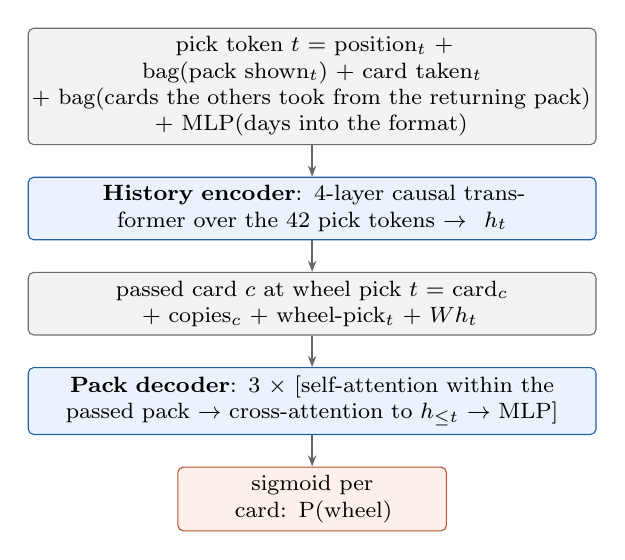
\begin{tikzpicture}[
  font=\footnotesize,
  box/.style={draw=#1!80!black,fill=#1!10,rounded corners=2pt,minimum height=0.55cm,inner sep=3pt,align=center,text width=7.0cm},
  box/.default=cgray,
  sm/.style={draw=#1!80!black,fill=#1!10,rounded corners=2pt,minimum height=0.55cm,inner sep=3pt,align=center,text width=3.2cm},
  arr/.style={-{Stealth[length=4pt]},draw=black!60,thick},
  node distance=0.4cm]
\node[box] (tok) {pick token $t$ = position$_t$ + bag(pack shown$_t$) + card taken$_t$\\
  + bag(cards the others took from the returning pack)\\ + MLP(days into the format)};
\node[box=cblue,below=of tok] (hist) {\textbf{History encoder}: 4-layer causal transformer over the 42 pick tokens $\to h_t$};
\node[box,below=of hist] (ctok) {passed card $c$ at wheel pick $t$ = card$_c$ + copies$_c$ + wheel-pick$_t$ + $W h_t$};
\node[box=cblue,below=of ctok] (cand) {\textbf{Pack decoder}: 3 $\times$ [self-attention within the passed pack $\to$ cross-attention to $h_{\le t}$ $\to$ MLP]};
\node[sm=corange,below=of cand] (out) {sigmoid per card: P(wheel)};
\draw[arr] (tok) -- (hist);
\draw[arr] (hist) -- (ctok);
\draw[arr] (ctok) -- (cand);
\draw[arr] (cand) -- (out);
\end{tikzpicture}
\caption{WheelNet. The history encoder summarises everything the drafter knows after pick $t$, including the
card they just took. Each card they pass at a wheel-eligible pick becomes a token that attends to the other
passed cards (which cards shield it) and to the history (which colours the table is taking), and gets an
independent probability of coming back. Card vectors are a learned per-card embedding plus a linear map of
colour, rarity and mana value.}
\label{fig:arch}
\end{figure}

WheelNet (Fig.~\ref{fig:arch}) has the same two halves as PickNet~\cite{picknet}: a causal history encoder and a
pack decoder. It is set up for a different question. The companion guide~\cite{wheelarch} walks through every
layer; we summarise here.

\textbf{Cards.} A card's vector is a learned 192-dimensional embedding plus a linear projection of 14 fixed
attributes (five colour flags, rarity one-hot, mana value, creature and bonus-sheet flags).

\textbf{History encoder.} Pick $t$ of the 42 (for 14-card packs) gets one token: a position embedding; a
projected, count-weighted mean of the cards in the pack shown at $t$; the card taken at $t$; a projected bag of
the cards the other seven took from the pack that has just returned (empty for the first 8 picks of each pack);
and, in the final model, an MLP of how many days into the format the draft is. Unlike PickNet, token $t$
includes the pick at $t$. The question is asked \emph{after} the drafter has picked, about the cards they pass.
Four pre-norm layers of causal self-attention give states $h_t$ that see packs and picks $\le t$ and nothing
later. In particular they never see the returning pack.

\textbf{Pack decoder.} At each of the 18 wheel-eligible picks, every distinct passed card becomes a token: its
card vector, an embedding of its copy count, an embedding of which wheel pick this is, and a projection of $h_t$.
Three decoder blocks alternate self-attention among the cards passed together, cross-attention to $h_0,\dots,h_t$
and an MLP. All 18 passed packs of a draft share one sequence of 234 slots, with a block-diagonal mask so
cards attend only within their own pack. A small head gives one logit per card, and the loss is binary
cross-entropy over every real passed card.

The decoder's self-attention matters because wheeling is a competition. A card survives if the seven picks go
to other cards in the pack, so its chance depends on what it is passed alongside. The GBM's \texttt{n\_better}
feature encodes the same idea by hand. The decoder learns it.

\textbf{Training.} $d=192$, 6 heads, 4 history layers, 3 pack blocks, dropout 0.2: 3.86M parameters. AdamW (weight
decay 0.01), batch 128 drafts, gradient clipping at 1, a one-cycle schedule peaking at $10^{-3}$ with 5\% warm-up.
We keep the epoch with the best validation log loss. MSH trains for 8 epochs (26 minutes on an Apple-silicon
laptop, PyTorch MPS). Other sets get $\mathrm{round}(8 \cdot 48\text{k} / \text{training drafts})$ epochs, clamped to
3--8, so each costs about the same.

\textbf{Features-only, many sets.} With \texttt{ids=False} a card has no learned vector. It is an MLP
(465 $\to$ 384 $\to$ 192) of a fixed 465-dimensional feature vector: the 14 attributes, card types,
Scryfall-derived rules features, and a 384-dimensional \texttt{bge-small-en-v1.5}~\cite{bge} embedding of
the rules text, as in PickNet. One set of weights then scores any set. We train it on 20k random drafts from
each of the 7 other 14-card sets with complete pick-1 data (OTJ, DSK, FDN, DFT, TDM, FIN, SOS), with or without
MSH's own training drafts, for 4 epochs (4.05M parameters, 48 minutes with MSH included).

% =====================================================================
\section{Results}\label{sec:results}

\begin{table}[t]
\centering\small
\caption{MSH test (10,292 drafts, 1.95M passed cards, base wheel rate 33.3\%). Each LightGBM row adds a feature
group. ``vs ALSA'': relative log-loss reduction. Bold: best.}
\label{tab:msh}
\setlength{\tabcolsep}{2.6pt}
\resizebox{\columnwidth}{!}{\begin{tabular}{lcccc}
\toprule
model & log loss & AUC & ECE & vs ALSA \\
\midrule
pick-number prior & .6067 & .639 & .000 & $-$31.1\% \\
ALSA/ATA logistic & .4629 & .831 & .007 & 0 \\
card $\times$ pick lookup & .4602 & .833 & .009 & +0.6\% \\
\midrule
GBM: card & .4588 & .834 & .008 & +0.9\% \\
GBM: card + pack & .4397 & .850 & .008 & +5.0\% \\
GBM: card + signals & .4496 & .842 & .006 & +2.9\% \\
GBM: card + pack + signals & .4315 & .857 & .005 & +6.8\% \\
\midrule
WheelNet & .4249 & .862 & \textbf{.002} & +8.2\% \\
WheelNet + days into format & .4218 & .864 & .007 & +8.9\% \\
WheelNet + GBM average & .4258 & .861 & .005 & +8.0\% \\
\midrule
features-only, 7 other sets (day zero) & .5245 & .776 & .048 & $-$13.3\% \\
\textbf{features-only, 7 other sets + MSH} & \textbf{.4188} & \textbf{.866} & .003 & \textbf{+9.5\%} \\
\bottomrule
\end{tabular}}
\end{table}

\textbf{Card identity is nearly exhausted by ALSA} (Table~\ref{tab:msh}). The empirical wheel rate of each card at
each pick improves on the ALSA/ATA regression by only 0.6\%, and a GBM on card features alone by 0.9\%. Whatever
a per-card statistic can say, ALSA mostly says.

\textbf{The pack is the biggest single lever.} Adding the pack features cuts log loss by another 4.1 points
(+5.0\% in total). The top two features by gain are \texttt{n\_better} and the pack's take mass: a card wheels when
the seven drafters have better things to take. Signals alone add 2.9\%, and they stack with the pack (+6.8\%).
The signal gain grows over the draft. Over the card$\times$pick lookup, the card + signals GBM gains 0.9\%, 2.0\%
and 4.0\% in packs 1, 2 and 3, while the pack features' gain stays flat (5.0\%, 4.2\%, 4.2\%). Earlier rounds
reveal more about the table. The fourth most useful feature is
the wheel surprise of the card's colours in earlier rounds.

\textbf{The raw history beats the hand-built features.} WheelNet, which sees no engineered features, reaches
0.4249 (+8.2\%) and is the best-calibrated model (ECE 0.002). Averaging it with the GBM makes things slightly
worse, so the GBM's features appear to be subsumed. Three changes took WheelNet from a tie with the GBM (an
earlier version scored 0.4316) to this result: cross-attention from each passed card to the history, instead of
one pooled state; explicit tokens for what the others took; and dropout 0.2 over 8 epochs. Going deeper (6
history and 4 pack layers) did not help.

\begin{table*}[t]
\centering\small
\caption{Test results by set (Premier Draft, last 15\% of drafts). GBM: LightGBM on card + pack + signal
features. WheelNet: the per-set model without draft context (the MSH row is the 0.4249 model of
Table~\ref{tab:msh}). \emph{Best card}: log-loss reduction against ALSA on the passed card with the lowest
training ATA in its pack. \emph{ECE, top 3}: mean calibration error on the three best passed cards.
Bold: better of ALSA, GBM and WheelNet.}
\label{tab:sets}
\setlength{\tabcolsep}{3.4pt}
\resizebox{\textwidth}{!}{\begin{tabular}{lrrrc ccc cc cc c cc}
\toprule
 & drafts & pack & test ex. & wheel & \multicolumn{3}{c}{log loss $\downarrow$} & \multicolumn{2}{c}{vs ALSA (\%) $\uparrow$} & \multicolumn{2}{c}{AUC $\uparrow$} & best card & \multicolumn{2}{c}{ECE, top 3 $\downarrow$} \\
\cmidrule(lr){6-8}\cmidrule(lr){9-10}\cmidrule(lr){11-12}\cmidrule(lr){13-13}\cmidrule(lr){14-15}
set & (k) & size & (M) & rate & ALSA & GBM & WheelNet & GBM & WheelNet & ALSA & WheelNet & vs ALSA (\%) & ALSA & WheelNet \\
\midrule
BLB & 155 & 13 & 3.46 & 0.300 & 0.4991 & 0.4691 & \textbf{0.4622} & +6.0 & \textbf{+7.4} & 0.783 & \textbf{0.821} & +11.6 & 0.017 & \textbf{0.005} \\
DFT & 141 & 14 & 4.00 & 0.333 & 0.4608 & 0.4266 & \textbf{0.4239} & +7.4 & \textbf{+8.0} & 0.832 & \textbf{0.862} & +13.7 & 0.019 & \textbf{0.005} \\
DSK & 168 & 14 & 4.73 & 0.334 & 0.4542 & 0.4191 & \textbf{0.4159} & +7.7 & \textbf{+8.4} & 0.838 & \textbf{0.868} & +14.2 & 0.018 & \textbf{0.004} \\
ECL & 99 & 13 & 2.06 & 0.290 & 0.4911 & 0.4648 & \textbf{0.4508} & +5.4 & \textbf{+8.2} & 0.785 & \textbf{0.826} & +12.8 & 0.018 & \textbf{0.003} \\
FDN & 131 & 14 & 3.69 & 0.334 & 0.4614 & 0.4241 & \textbf{0.4202} & +8.1 & \textbf{+8.9} & 0.832 & \textbf{0.865} & +16.6 & 0.021 & \textbf{0.004} \\
FIN & 140 & 14 & 3.98 & 0.333 & 0.4771 & 0.4420 & \textbf{0.4375} & +7.4 & \textbf{+8.3} & 0.820 & \textbf{0.853} & +14.4 & 0.025 & \textbf{0.007} \\
LCI & 135 & 15 & 4.68 & 0.364 & 0.4860 & 0.4484 & \textbf{0.4434} & +7.7 & \textbf{+8.8} & 0.824 & \textbf{0.858} & +14.5 & 0.029 & \textbf{0.009} \\
MKM & 158 & 13 & 3.53 & 0.300 & 0.4814 & 0.4519 & \textbf{0.4487} & +6.1 & \textbf{+6.8} & 0.802 & \textbf{0.833} & +12.8 & 0.021 & \textbf{0.004} \\
MSH & 69 & 14 & 1.95 & 0.333 & 0.4629 & 0.4315 & \textbf{0.4249} & +6.8 & \textbf{+8.2} & 0.831 & \textbf{0.862} & +14.1 & 0.024 & \textbf{0.004} \\
OTJ & 195 & 14 & 5.51 & 0.334 & 0.4472 & 0.4085 & \textbf{0.4058} & +8.7 & \textbf{+9.3} & 0.845 & \textbf{0.876} & +16.7 & 0.026 & \textbf{0.008} \\
SOS & 107 & 14 & 3.05 & 0.333 & 0.4691 & 0.4284 & \textbf{0.4150} & +8.7 & \textbf{+11.5} & 0.824 & \textbf{0.869} & +14.8 & 0.021 & \textbf{0.003} \\
TDM & 101 & 14 & 2.87 & 0.333 & 0.4574 & 0.4262 & \textbf{0.4177} & +6.8 & \textbf{+8.7} & 0.840 & \textbf{0.869} & +14.5 & 0.021 & \textbf{0.003} \\
TLA & 103 & 14 & 2.71 & 0.324 & 0.4596 & 0.4267 & \textbf{0.4214} & +7.2 & \textbf{+8.3} & 0.829 & \textbf{0.861} & +13.4 & 0.021 & \textbf{0.002} \\
TMT & 32 & 14 & 0.84 & 0.325 & 0.4625 & 0.4250 & \textbf{0.4173} & +8.1 & \textbf{+9.8} & 0.829 & \textbf{0.866} & +16.1 & 0.025 & \textbf{0.005} \\
\midrule
mean & & & & 0.326 & 0.4693 & 0.4352 & \textbf{0.4289} & +7.3 & \textbf{+8.6} & 0.822 & \textbf{0.856} & +14.3 & 0.022 & \textbf{0.005} \\
\bottomrule
\end{tabular}
}
\end{table*}

\begin{figure}[t]
\centering
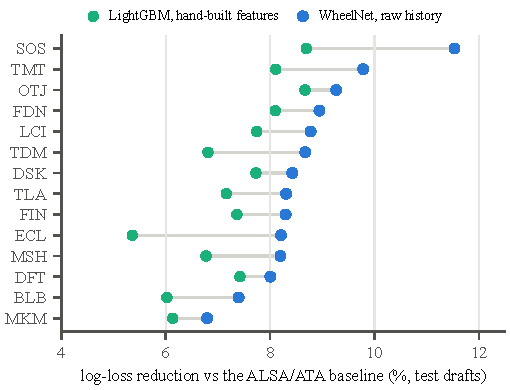
\includegraphics[width=\columnwidth]{figs/per_set.pdf}
\caption{Log-loss reduction against ALSA/ATA by set, sorted by WheelNet. Grey lines join each set's GBM to its
WheelNet.}
\label{fig:sets}
\end{figure}

\textbf{It holds on every set} (Table~\ref{tab:sets}, Fig.~\ref{fig:sets}). Across 14 sets WheelNet cuts log loss
by 8.6\% on average against ALSA (6.8\% on MKM to 11.5\% on SOS), and the GBM by 7.3\%. WheelNet wins on all 14,
by 0.6--2.8 points. AUC rises from 0.822 to 0.856 on average. The 13-card sets (BLB, ECL, MKM) have the lowest AUCs for
every model.

\textbf{Pretraining on other sets is best.} The features-only model trained on 7 other sets plus MSH's training
drafts reaches 0.4188 (+9.5\%, AUC 0.866), better than the per-set WheelNet with the same inputs. PickNet found the
same~\cite{picknet}: cards seen through shared features generalise better than one set's learned identities. We
have this model for MSH only.

\textbf{Day zero is far behind ALSA.} Trained only on the 7 other sets, the model scores 0.5245 on MSH. It closes
57\% of the gap from the pick prior to ALSA. It knows how tables behave but not how good the new set's cards are,
and it is miscalibrated (ECE 0.048). A few days of a set's own data, enough to fit ALSA, beat it.

\textbf{What WheelNet needs to know.} An input ablation on MSH validation (8 epochs each) found one useful extra
input: days into the format ($-$0.0039 log loss). Rank and 17Lands skill buckets added nothing ($+$0.0003), since
the drafter's picks already show how they draft. Card types were a wash ($-$0.0004). On test, WheelNet with time
scores 0.4218 (+8.9\%), at some cost in calibration (ECE 0.007).

% =====================================================================
\section{Where it matters: the cards you want back}\label{sec:where}

\begin{figure}[t]
\centering
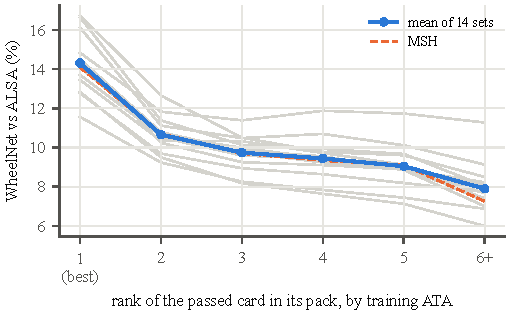
\includegraphics[width=\columnwidth]{figs/by_rank.pdf}
\caption{WheelNet's log-loss reduction against ALSA by the passed card's rank in its pack (1 = the best card
passed, by training ATA). Grey: each of the 14 sets.}
\label{fig:rank}
\end{figure}

Most passed cards are chaff, which obviously wheels. The useful question is whether the \emph{second-best}
card, the one passed when you take the best, will come back. We rank each passed card within its pack by training ATA.
Rank 1 is the best card passed.

\textbf{The model earns most where it matters} (Fig.~\ref{fig:rank}). On every set the gain over ALSA is largest
for the best passed card, 11.6--16.7\% (mean 14.3\%), and it falls with rank to 7.9\% for ranks 6 and below.
Whether a good card survives depends on the table more than on the card.

\begin{figure}[t]
\centering
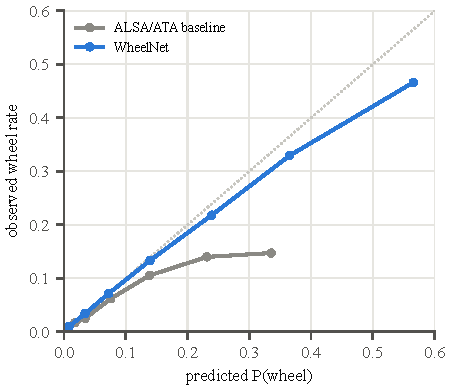
\includegraphics[width=0.88\columnwidth]{figs/calib_rank2.pdf}
\caption{Calibration on the second-best passed card, MSH test (185k cards). Bins at 2, 5, 10, 20, 30 and 50\%;
bins with fewer than 200 cards are dropped. ALSA's high predictions come true half as often as it says.}
\label{fig:calib}
\end{figure}

\textbf{ALSA is overconfident about your good cards} (Fig.~\ref{fig:calib}). It is calibrated on average (ECE
0.007 on MSH), but on the top three passed cards its ECE is 0.017--0.029 across sets, against 0.002--0.009 for
WheelNet, 3--10$\times$ worse. On MSH, when ALSA gives the second-best passed card a 30--50\% chance, it comes back
15\% of the time. In WheelNet's 30--50\% bin it comes back 33\% of the time. ALSA is a per-card average over every pack the card
appears in. Being the best card \emph{you} pass usually means the pack is thin, with little else to absorb the
seven picks, so the card's chance of lasting is lower than its average.

\textbf{For a top-3 card the answer is almost always ``no''.} WheelNet puts at least 50\% on 0.3\% of them. Its
value is in separating 1\% from 25\%. On MSH it gives a quarter of second-best cards under 2\%, and 1.0\% of those
wheel. The 7.5\% it puts above 20\% wheel 25\% of the time.

% =====================================================================
\section{Staying current}\label{sec:temporal}

\begin{figure}[t]
\centering
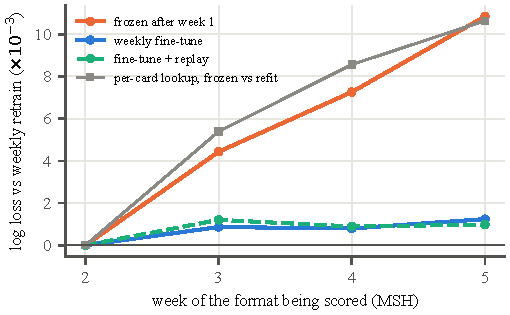
\includegraphics[width=\columnwidth]{figs/temporal.pdf}
\caption{MSH weekly walk-forward. Each week is scored by models trained only on earlier weeks. Lines show log
loss against a model retrained from scratch on all earlier weeks; grey compares a per-card lookup frozen after
week 1 with one refitted weekly.}
\label{fig:temporal}
\end{figure}

A format changes after release: drafters learn which cards are good, and what they take changes what
wheels. We split MSH into weeks (27.7k, 15.7k, 11.4k, 10.2k and 3.6k drafts, with thin trailing weeks merged) and
score each week $w \ge 2$ with models trained only on weeks before it (Fig.~\ref{fig:temporal}). The model is
WheelNet with days-into-format.

\textbf{A frozen model goes stale, and the gap grows.} Trained on week 1 and never updated, WheelNet falls behind
a weekly retrain by 0.0044, 0.0073 and 0.0108 log loss in weeks 3, 4 and 5. The frozen per-card lookup decays in
the same way (0.466 $\to$ 0.469) while a refitted one improves. By week 5 the staleness costs more than WheelNet's
whole advantage over the GBM on the test set (0.0066).

\textbf{A weekly fine-tune is enough.} Two epochs on the latest week alone, at learning rate $3\times10^{-4}$, stay
within 0.0008--0.0012 of a full retrain. Mixing an equal sample of older drafts into the fine-tune (replay) adds
nothing.

% =====================================================================
\section{Does the open lane pay?}\label{sec:lane}

\begin{table*}[t]
\centering\small
\caption{Open-lane analysis by set (all Premier drafts). \emph{Persistence}: correlation of a colour's openness
between packs (P1 and P3 share the upstream neighbour). \emph{Follow slope}: change in the log-odds that a
colour is one of the drafter's two main colours per sd of its P1 openness. \emph{Payoff}: log-odds of winning
a game per sd of P1 openness of the main colours, with pair, rank and skill controls ($\pm$ s.e.). \emph{Other
colours}: payoff of P1 openness in the three colours the drafter did not play, fitted jointly with their main
colours.}
\label{tab:lane}
\setlength{\tabcolsep}{4.5pt}
\resizebox{\textwidth}{!}{\begin{tabular}{lr cc c c c c c}
\toprule
 & drafts & \multicolumn{2}{c}{persistence (corr.)} & follow & follow slope & payoff per sd & game win \% by & payoff, \\
\cmidrule(lr){3-4}
set & (k) & P1--P3 & P1--P2 & slope & bronze $\to$ mythic & (+ skill) & P1 quintile 1 $\to$ 5 & other colours \\
\midrule
BLB & 155 & 0.218 & 0.084 & 0.33 & 0.30 $\to$ 0.36 & +0.056 $\pm$ 0.003 & 53.1 $\to$ 56.2 & $+$0.003 \\
DFT & 141 & 0.246 & 0.102 & 0.37 & 0.32 $\to$ 0.39 & +0.060 $\pm$ 0.003 & 53.2 $\to$ 56.6 & $+$0.004 \\
DSK & 168 & 0.236 & 0.087 & 0.37 & 0.36 $\to$ 0.39 & +0.057 $\pm$ 0.003 & 53.0 $\to$ 56.2 & 0.000 \\
ECL & 99 & 0.234 & 0.114 & 0.35 & 0.32 $\to$ 0.37 & +0.065 $\pm$ 0.004 & 52.7 $\to$ 56.5 & $-$0.012 \\
EOE & 104 & 0.259 & 0.096 & 0.41 & 0.37 $\to$ 0.44 & +0.056 $\pm$ 0.004 & 53.5 $\to$ 56.6 & $+$0.012 \\
FDN & 131 & 0.238 & 0.088 & 0.37 & 0.32 $\to$ 0.43 & +0.063 $\pm$ 0.003 & 52.9 $\to$ 56.5 & $-$0.005 \\
FIN & 140 & 0.225 & 0.090 & 0.36 & 0.31 $\to$ 0.40 & +0.059 $\pm$ 0.003 & 53.4 $\to$ 57.0 & $-$0.004 \\
LCI & 135 & 0.177 & 0.062 & 0.33 & 0.28 $\to$ 0.37 & +0.052 $\pm$ 0.003 & 54.1 $\to$ 57.0 & $-$0.002 \\
MKM & 158 & 0.203 & 0.068 & 0.34 & 0.29 $\to$ 0.38 & +0.049 $\pm$ 0.003 & 53.8 $\to$ 56.6 & $+$0.007 \\
MSH & 69 & 0.234 & 0.106 & 0.36 & 0.33 $\to$ 0.39 & +0.057 $\pm$ 0.005 & 54.0 $\to$ 57.3 & $-$0.013 \\
OTJ & 195 & 0.179 & 0.056 & 0.33 & 0.28 $\to$ 0.36 & +0.050 $\pm$ 0.003 & 52.7 $\to$ 55.6 & $+$0.005 \\
SOS & 107 & 0.234 & 0.120 & 0.37 & 0.32 $\to$ 0.40 & +0.057 $\pm$ 0.004 & 53.4 $\to$ 56.9 & $-$0.015 \\
TDM & 101 & 0.183 & 0.065 & 0.35 & 0.31 $\to$ 0.36 & +0.052 $\pm$ 0.004 & 53.3 $\to$ 56.4 & $-$0.004 \\
TLA & 103 & 0.229 & 0.097 & 0.37 & 0.33 $\to$ 0.39 & +0.049 $\pm$ 0.004 & 54.4 $\to$ 56.9 & $+$0.009 \\
TMT & 32 & 0.236 & 0.100 & 0.35 & 0.29 $\to$ 0.37 & +0.047 $\pm$ 0.007 & 55.7 $\to$ 58.5 & $-$0.018 \\
\midrule
mean & & 0.222 & 0.089 & 0.36 & 0.32 $\to$ 0.39 & +0.055 & 53.5 $\to$ 56.7 & $-$0.002 \\
\bottomrule
\end{tabular}
}
\end{table*}

The repository's namesake question is whether reading an open lane pays. WheelNet reads signals well (\S\ref{sec:results}),
so they exist. Do drafters use them, and does it help?

\textbf{Openness.} For pack $k$ and colour $j$, openness is the total of good cards of colour $j$ that reached
the drafter later than they usually last:
\[
\text{flow}_{kj} = \sum_{q=1}^{7} \sum_{c \in \mathbf{s}_q} \text{share}_{cj} \cdot \max(0,\, q - \text{ALSA}_c),
\]
where share$_{cj}$ splits a multicolour card evenly across its colours. Picks 8 and later are excluded, since
those packs have been round the whole table. We z-score flow per pack and colour within each draft week, so
set-wide shifts in colour popularity cancel. The drafter's own picks never enter it: openness is fixed by the
opened packs and the upstream drafters. A drafter's \emph{main colours} are the top two by playability-weighted
picks.

\textbf{Signals are real and travel through your neighbour} (Table~\ref{tab:lane}). Packs pass left in P1 and P3
and right in P2, so P1 and P3 have the same upstream neighbour. A colour's P1 openness correlates 0.22 with its P3
openness and 0.09 with its P2 openness, on every set. P1 does tell you about P3.

\textbf{Drafters follow, and better drafters follow more.} One sd of P1 openness raises the log-odds that the
colour ends up a main colour by 0.36. The slope rises with rank, from 0.32 for bronze to 0.39 for mythic (mean
over sets), and with the 17Lands win-rate bucket, from 0.32 to 0.39, on all 15 sets. Still, only 17\% of drafters
end in the most open P1 pair, against 10\% by chance.

\begin{figure}[t]
\centering
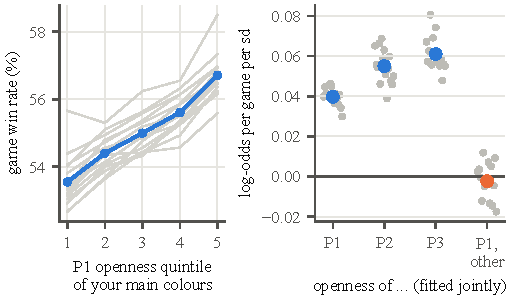
\includegraphics[width=\columnwidth]{figs/open_lane.pdf}
\caption{Left: game win rate by quintile of P1 openness of the drafter's main colours (grey: each of 15 sets).
Right: payoff per sd of openness when P1, P2 and P3 openness of the main colours, or P1 openness of the main and
other colours, are fitted jointly, with skill controls (grey: sets).}
\label{fig:lane}
\end{figure}

\textbf{Open colours win games.} We fit a binomial logit to each draft's game record ($p^W(1-p)^L$) with
colour-pair fixed effects, rank and the 17Lands skill bucket. One sd of openness in the main colours is worth
+0.055 log-odds per game (s.e.\ 0.003--0.007 per set, positive on 15/15 sets). From the bottom quintile to the top, game win rate
rises by 3.2 points, 53.6\% to 56.7\% (Fig.~\ref{fig:lane}, left). Drafters who end in the most open P1 pair win
0.9--1.9 points more games.

\textbf{But the payoff is supply, not the read.} If reading the lane were what paid, openness you can read before
committing should matter most. It doesn't (Fig.~\ref{fig:lane}, right). Fitted jointly, P2 openness, which arrives
after most drafters have committed, pays as much as P1 openness (+0.055 vs +0.040), and P3 pays most (+0.061).
Holding the main colours' openness fixed, openness in the colours the drafter did \emph{not} take has no effect
($-$0.002 on average, negative on only 9 of 15 sets). More good cards in your colours win games, whenever they
arrive. That is the reason to read signals, but this data cannot separate the value of the decision from the
luck of the seat.

\begin{table}[t]
\centering\small
\caption{Follow or force? Seat 0's deck score (mean GIH WR, \%, of the best colour pair's 23 best cards) over
2,000 simulated tables of real opened test packs. Seats 1--7 are PickNet bots in every arm. $\Delta$: difference
from \emph{follow}, paired on the same tables ($\pm$ s.e.).}
\label{tab:force}
\setlength{\tabcolsep}{3.0pt}
\resizebox{\columnwidth}{!}{\begin{tabular}{lcccc}
\toprule
 & \multicolumn{2}{c}{MSH} & \multicolumn{2}{c}{FDN} \\
\cmidrule(lr){2-3}\cmidrule(lr){4-5}
seat 0 strategy & score & $\Delta$ & score & $\Delta$ \\
\midrule
follow (draft like a human) & 57.36 & --- & 55.78 & --- \\
force a random pair & 57.39 & +0.02 $\pm$ .03 & 55.78 & $-$0.00 $\pm$ .02 \\
force the best pair & 58.67 & +1.30 & 56.26 & +0.48 \\
read P1 picks 1--5, then lock & 56.94 & $-$0.42 $\pm$ .03 & 55.52 & $-$0.26 $\pm$ .02 \\
\bottomrule
\end{tabular}}
\end{table}

\textbf{Counterfactual: follow or force?} To separate the read from the seat, we use a table simulator built
on per-set PickNet models~\cite{picknet}. Eight bots draft a test drafter's real opened packs, and each samples
its pick from the model's softmax. Seats 1--7 always draft like humans. Seat 0 plays a strategy, with the same
tables and random stream for every strategy. \emph{Follow} drafts like a human, reading signals as people do.
\emph{Force} samples from the same model restricted to cards that fit a fixed pair, assigned round-robin
across tables. \emph{Read-then-lock} drafts freely for P1 picks 1--5, then locks the pair with the most openness
so far. Pools are scored as decks: for each pair, the mean GIH WR (from training games) of the 23 best cards that
fit, with missing slots filled by a 10th-percentile card. The score is the best pair's.

\textbf{Forcing a random pair ties drafting like a human} (Table~\ref{tab:force}), on both sets, within
$\pm$0.03 points. Which pair matters much more than when you commit. Forcing the best pair (WU in MSH, WB in
FDN) beats following by 1.30 and 0.48 points, and 2.9 points separate the best and worst pair to force in MSH
(0.9 in FDN, a flatter format). Locking in whatever looks open after five picks, ignoring the cards already
taken, is worse than both ($-$0.42 and $-$0.26). Human-style drafting balances card quality, pool and signals;
pure signal-chasing gives up the first two.

% =====================================================================
\section{Limitations}

\begin{itemize}
\item \textbf{One seat, 17Lands users.} We see one drafter per table, and 17Lands users are above the Arena average.
The wheel model describes what happens around a 17Lands user. A table of weaker drafters will behave
differently.
\item \textbf{Single runs, one development set.} Each number is one seed. The architecture search, input ablation,
pretraining and walk-forward were run on MSH only. The per-set WheelNet on the other 13 sets lacks the time
input and pretraining, so it understates the best model.
\item \textbf{Leaky card statistics in the GBM.} ATA, ALSA and wheel rates are fitted on the same training rows
the GBM learns from. With about 27k examples per card the leak is small, but out-of-fold encoding would be
cleaner. WheelNet is unaffected.
\item \textbf{Observational payoff.} The skill bucket that controls for drafter quality is computed over the
drafter's whole history on the set, including the outcome. Controlling for it removes about an eighth of the raw effect (+0.064 $\to$ +0.055).
\item \textbf{Simulated tables.} The bots imitate 17Lands users, not strong drafters. They under-draft WU (17\%
of bot decks against 23\% of real MSH drafters), so a WU forcer meets less competition than at a real table.
The deck score ignores curve and synergy, and every forcing seat is alone. Tables where several seats force
are untested.
\end{itemize}

\section{Conclusion}

Whether a passed card comes back depends far more on what it is passed with, and on what the table has been
taking, than on the card. A transformer that reads the raw draft, including what the other seven took from each
returning pack, predicts it better than hand-built features on every set we tried. It does best on the good cards
drafters plan around, where the standard per-card statistic is overconfident. It needs a weekly refresh to stay
ahead. The signals it reads are real, drafters act on them, and open colours win games. But the value of an open
lane is in the cards that arrive, and in simulation committing to a pair early costs nothing. Code and results
are available at \url{https://github.com/zscore/wheelnet}.

\small
\begin{thebibliography}{99}\setlength{\itemsep}{1pt}
\bibitem{17lands} 17Lands. Public datasets. \url{https://www.17lands.com/public_datasets}.
\bibitem{overlay} MTGA\_Draft\_17Lands: a draft overlay for MTG Arena using 17Lands data.
\url{https://github.com/bstaple1/MTGA_Draft_17Lands}.
\bibitem{17landssim} 17Lands. Simulating draft strategies. 17Lands blog.
\bibitem{ward2021} H.~N. Ward, B.~Mills, D.~J. Brooks, A.~S. Khakhalin, D.~Troha. AI solutions for drafting in
\emph{Magic: the Gathering}. \emph{IEEE Conference on Games}, 2021. arXiv:2009.00655.
\bibitem{bertram2021} T.~Bertram, J.~F\"urnkranz, M.~M\"uller. Predicting human card selection in
\emph{Magic: The Gathering} with contextual preference ranking. \emph{IEEE CoG}, 2021. arXiv:2105.11864.
\bibitem{bertram2024infonce} T.~Bertram, J.~F\"urnkranz, M.~M\"uller. Contrastive learning of preferences
with a contextual InfoNCE loss. arXiv:2407.05898, 2024.
\bibitem{draftfm} B.~Ward. DraftFM: a foundation model for day-zero drafting in \emph{Magic: The Gathering}.
arXiv:2608.19568, 2026.
\bibitem{puder} P.~Czerner. puder: an AI for MTG drafting. \url{https://nicze.de/philipp/articles/puder/}, 2025;
code at \url{https://github.com/suyjuris/puder}.
\bibitem{picknet} Z.~Blanton. PickNet: one transformer for human draft picks in \emph{Magic: The Gathering},
trained on 17 sets. Technical report, 2026. \url{https://github.com/zscore/picknet}.
\bibitem{wheelarch} Z.~Blanton. How WheelNet works: a step-by-step guide to the architecture. Companion to this
report, 2026.
\bibitem{draftencoder} A.~Rigaux, H.~Kashima. Predicting drafted deck strength for \emph{Magic: The
Gathering}. \emph{IEEE CoG}, 2026. arXiv:2607.04782.
\bibitem{lightgbm} G.~Ke, Q.~Meng, T.~Finley, T.~Wang, W.~Chen, W.~Ma, Q.~Ye, T.-Y.~Liu. LightGBM: a highly
efficient gradient boosting decision tree. \emph{NeurIPS}, 2017.
\bibitem{bge} S.~Xiao, Z.~Liu, P.~Zhang, N.~Muennighoff. C-Pack: packaged resources to advance general Chinese
embedding. arXiv:2309.07597, 2023.
\end{thebibliography}

\end{document}
